\chapter{Introduction Problem Statement; Literature Review}
\label{ch1}

\section{Problem Statement}
\subsection{This effort performs an ensemble study of ML architectures/parameters to best forecast 4 hours of turbulence conditions from prior measurements.}

\subsection{What is turbulence ($C_{n}^{2}$)? Why is it important to measure/model?}
\begin{figure}[h!]
	\centering
	\subfloat[Low-strength ($C_{n}^{2}$)\label{fig:first_frames_a}]{
		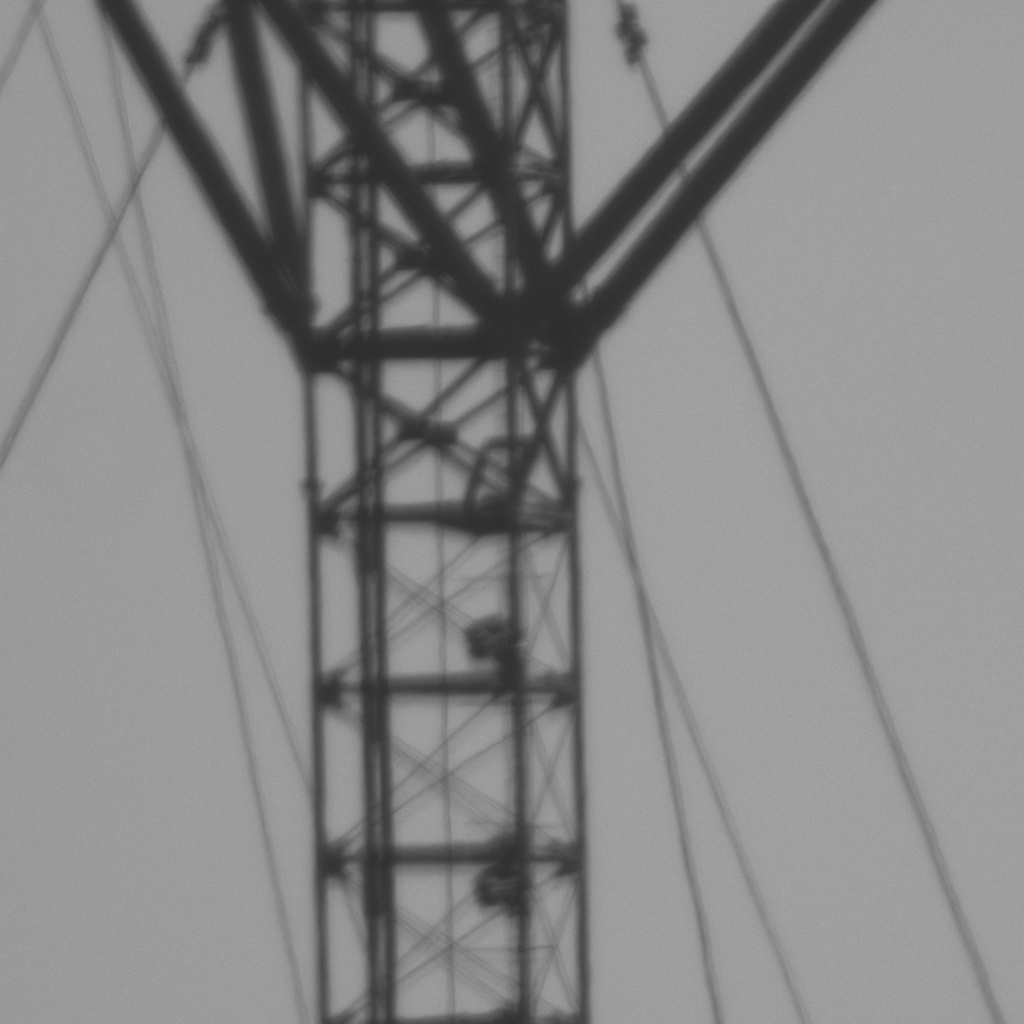
\includegraphics[width=0.49\textwidth]
		{FirstFrame_LowTurb.jpg}
	}
	\subfloat[High-strength ($C_{n}^{2}$)\label{fig:first_frames_b}]{
		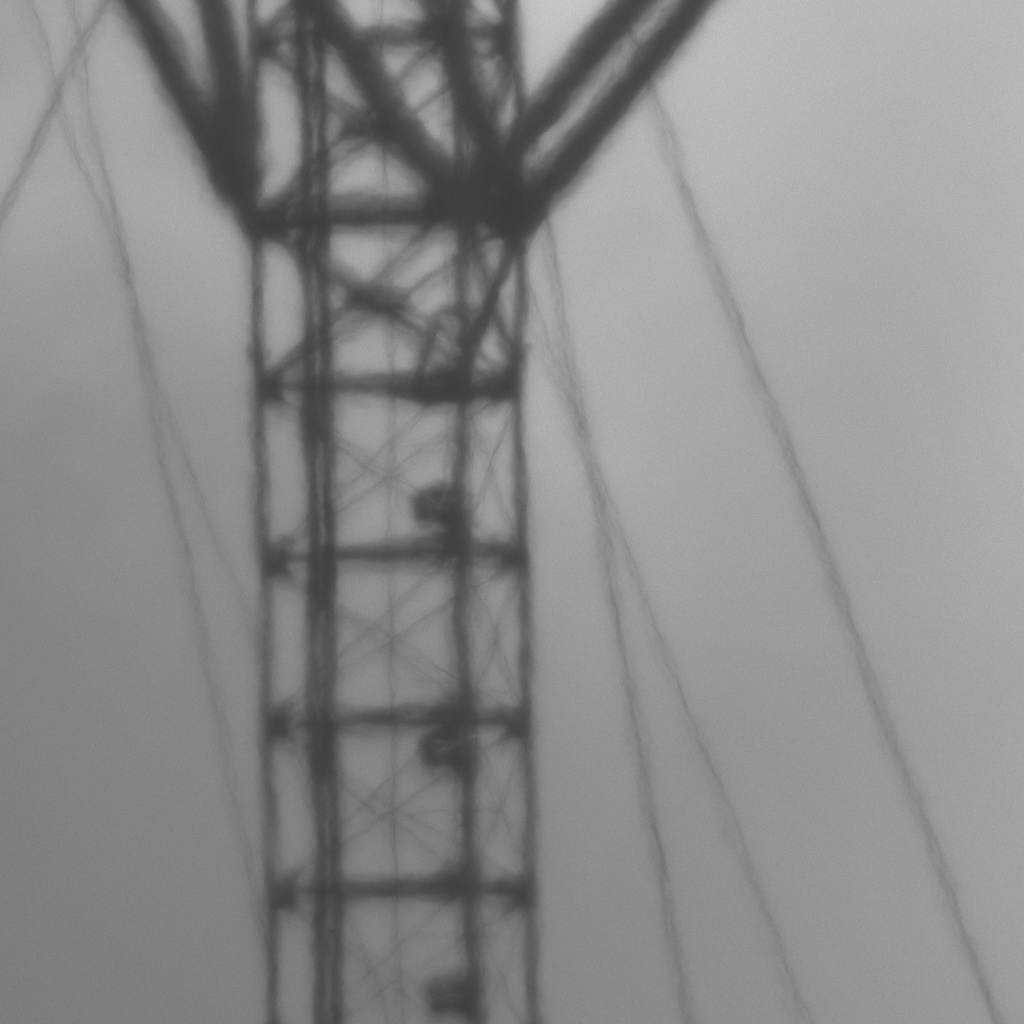
\includegraphics[width=0.49\textwidth]
		{FirstFrame_HighTurb.jpg}
	}
	\hfill
	\caption{Effect of low-strength and high-strength $C_{n}^{2}$ conditions.}
	\label{fig:first_frames}
\end{figure}

\subsection{Review the fundamentals of machine learning.}
Optimization algorithm!
\begin{figure}[h!]
	\centering
	\subfloat[Training\label{fig:simple_model_training_testing_a}]{
		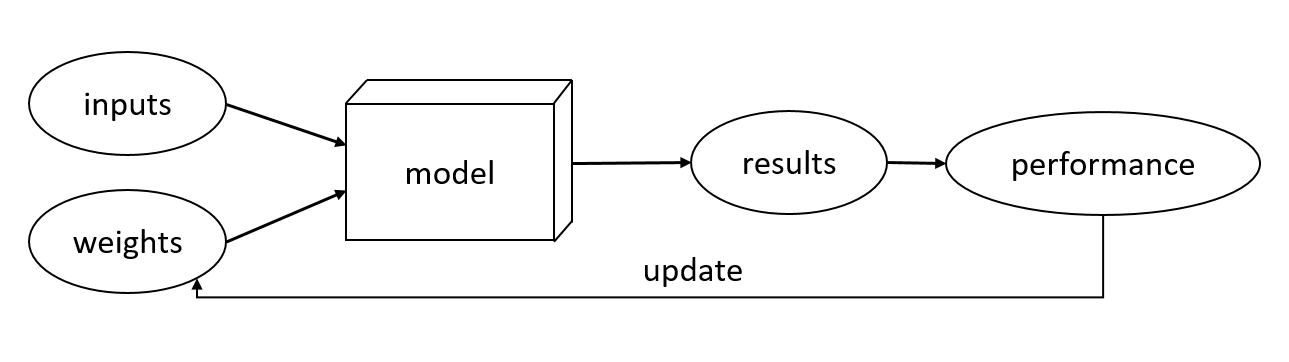
\includegraphics[width=0.99\textwidth]
		{training_process.png}
	}
	\hfill
	\subfloat[Testing\label{fig:simple_model_training_testing_b}]{
		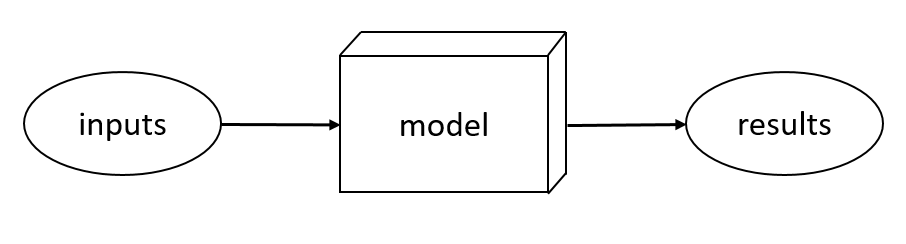
\includegraphics[width=0.99\textwidth]
		{testing_process.png}
	}
	\hfill
	\caption{Simple example of machine learning model training and testing.}
	\label{fig:simple_model_training_testing}
\end{figure}

\section{Literature Review}
\subsection{State of Turbulence $C_{n}^{2}$ Modeling}
\subsubsection{Physical Models}
\subsubsection{ML Models}
Recently published literature predicts $C_{n}^{2}$ conditions at time \textit{t} given weather inputs at time \textit{t}.
\subsection{General information about MLP/RNN architectures here? Does the in-depth review of the architectures go here?}